\subsection{Extraction de séquences}

Pour cette première partie, seul quelques extraits de codes seront présentés. L'intégralité du code source se trouve dans le fichier \texttt{src/hmmPart1.r} du projet. 

\subsubsection*{Extension de la fonction \texttt{simu\_symbol}}

La fonction \texttt{simu\_symbol} permet de construire et d'afficher des chiffres. Pour cela, elle récupère un ensemble de 30 points différents, qu'elle relie ensuite dans un odre précis. L'extension de cette fonction par le code ci-dessous, permet désormais de construire le chiffre 6.

\begin{lstlisting}
simu_symbol <- function()
{
	(...)
	digit_6 <- rbind(
		stroke(-0.5,1.0,-0.5,-0.5,10),
		stroke(-0.4,-0.5,0.5,-0.5,7),
		stroke(0.5,-0.4,0.5,0.4,6),
		stroke(0.4,0.4,-0.5,0.4,7)
	)
  dimnames(digit_6) <- list(num=1:nrow(digit_6),point=c("x","y"))
  plot(digit_6,type="l",col="red",xlim=c(-1,1),ylim=c(-1,1))
  points(digit_6)
  return(list(d1=digit_1,d2=digit_4,d3=digit_6))
}
\end{lstlisting}

\subsubsection*{Analyse de la fonction \texttt{compute\_symbol}}
La fonction \texttt{compute\_symbol} prend trois paramêtres en entrée : le tracé d'un chiffre, un nombre de lignes (5) et un nombre de colonnes (3). Elle commence par construire une matrice, ayant pour dimmension le nombre de lignes et de colonnes précisés précédemment. Cette matrice servira à positionner les points du tracé analysé :
\begin{center}
	$\begin{pmatrix}
		13 & 14 & 15 \\
		10 & 11 & 12 \\
		7 & 8 & 9 \\
		4 & 5 & 6 \\
		1 & 2 & 3
	\end{pmatrix}$
\end{center}

Elle calcule ensuite le nombre de points présents dans le tracé du chiffre, puis les positions horizontales et verticales de chacun de ces points. Pour finir, elle détermine la position de chaque point dans la matrice qu'elle a créée, et les affiche.\\

Voici les resultats donnés par cette fonction pour les trois tracés créés par la fonction \texttt{simu\_symbol} :
\begin{lstlisting}
	pour 1 : 11 11 14 14 14 14 14 14 14 14 14 14 14 14 11 11 11 11 8 8 8 8 5 5 5 5 2 2 2 2 
	pour 4 : 14 14 14 11 11 10 7 7 7 4 4 4 4 4 5 8 8 8 9 9 8 8 8 5 5 5 2 2 2 2 
	pour 6 : 13 13 13 10 10 7 7 7 4 4 4 5 5 5 5 6 6 6 6 9 9 12 12 12 11 11 11 11 10 10 
\end{lstlisting}
Ce qui donne pour le chiffre "6", les positions suivantes :
\begin{center}
	$\begin{pmatrix}
		 \textcolor{red}{13} & 14 & 15 \\
		\textcolor{red}{10} & \textcolor{red}{11} & \textcolor{red}{12} \\
		\textcolor{red}{7} & 8 & \textcolor{red}{9} \\
		\textcolor{red}{4} & \textcolor{red}{5} & \textcolor{red}{6} \\
		1 & 2 & 3
	\end{pmatrix}$
\end{center}

Avec une matrice contenant suffisamment de lignes et de colonnes, cette méthode permet de déterminer efficacement la position de chaque point d'un caractère. Cependant, si le caractère analysé est mal positionné (décalage à gauche ou à droite), toutes les positions sont également décalées au niveau de la matrice. Il faut donc faire un gros prétraitement pour que le caractère soit bien découpé et bien positionné. De plus, l'ordre de chaque points est essentiel pour la construction de la séquence.

\subsubsection*{Analyse de la fonction \texttt{compute\_symbol\_dir}}
La fonction \texttt{compute\_symbol\_dir} prend deux paramêtres en entrée : le tracé d'un chiffre et un nombre d'angles qui serviront de direction (ici 8). Chaque direction est numérotées telles que :
\begin{center}
	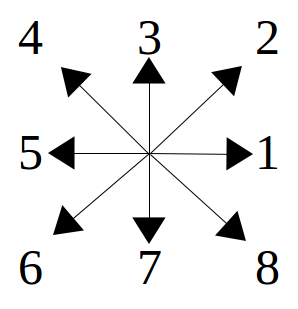
\includegraphics[width=0.20\textwidth]{Figures/direction.jpg}
\end{center}
Ainsi, la direction 1 indique un déplacement vers la droite, la direction 5 vers la gauche, etc\dots \\

Voici les resultats donnés par cette fonction pour les trois tracés créés par la fonction \texttt{simu\_symbol\_dir} :
\begin{lstlisting}
	pour 1 : 2 2 2 2 2 2 2 2 2 7 7 7 7 7 7 7 7 7 7 7 7 7 7 7 7 7 7 7 7 7 
	pour 4 : 6 6 6 6 6 6 6 6 6 5 1 1 1 1 1 1 1 1 1 4 7 7 7 7 7 7 7 7 7 7 
	pour 6 : 7 7 7 7 7 7 7 7 7 1 1 1 1 1 1 1 3 3 3 3 3 3 5 5 5 5 5 5 5 5 
\end{lstlisting}
Ce qui donne pour le chiffre "1" deux tracés : le premier allant vers le 2 et le second allant vers le 7.
\begin{center}
	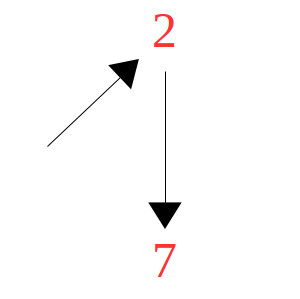
\includegraphics[width=0.20\textwidth]{Figures/direction_results.jpg}
\end{center}

L'un des principaux avantages de cette méthode est que la taille de la séquence, ainsi que sa position (avec ou sans décalage) n'affectent pas les résultats. Cette fonction arrive à déterminer précisément l'angle de la direction du tracé. Cependant, si l'image n'est pas dans le bon sens ou si l'écriture est inclinée ou en italique, la reconnaissance de l'angle sera faussée. De plus, le chiffre "1" et le chiffre "7" peuvent être facilement confondu à cause de certaines polices d'écriture. L'ordre de chaque points est également essentiel pour la construction de la séquence.


\subsection{Création et initialisation d'un HMM}

Pour cette nouvelle partie, nous considérerons un HMM à 3 états ($S_x$), observant 10 chiffres ($c_x$) et une topologie gauche-droite :
\begin{center}
	\begin{tikzpicture}
	 	% states
		\node[state] (s1) at (1,2) {$S_1$}
			edge [loop above] node[auto] {0.9} ();
		\node[state] (s2) at (4.5,2) {$S_2$}
			edge [<-,bend left=0] node[auto] {0.1} (s1)
			edge [loop above] node[auto] {0.9} ();
		\node[state] (s3) at (8,2) {$S_3$}
			edge [<-,bend left=0] node[auto] {0.1}  (s2)
			edge [loop above] node[auto] {1} ();
		% observations
		\node[observation] (c0) at (0,0) {$c_0$}
			edge [lightedge] (s1)
			edge [lightedge] (s2)
			edge [lightedge] (s3);
		\node[observation] (c1) at (1,0) {$c_1$}
			edge [lightedge] (s1)
			edge [lightedge] (s2)
			edge [lightedge] (s3);
		\node[observation] (c2) at (2,0) {$c_2$}
			edge [lightedge] (s1)
			edge [lightedge] (s2)
			edge [lightedge] (s3);
		\node[observation] (c3) at (3,0) {$c_3$}
			edge [lightedge] (s1)
			edge [lightedge] (s2)
			edge [lightedge] (s3);
		\node[observation] (c4) at (4,0) {$c_4$}
			edge [lightedge] (s1)
			edge [lightedge] (s2)
			edge [lightedge] (s3);
		\node[observation] (c5) at (5,0) {$c_5$}
			edge [lightedge] (s1)
			edge [lightedge] (s2)
			edge [lightedge] (s3);
		\node[observation] (c6) at (6,0) {$c_6$}
			edge [lightedge] (s1)
			edge [lightedge] (s2)
			edge [lightedge] (s3);
		\node[observation] (c7) at (7,0) {$c_7$}
			edge [lightedge] (s1)
			edge [lightedge] (s2)
			edge [lightedge] (s3);
		\node[observation] (c8) at (8,0) {$c_8$}
			edge [lightedge] (s1)
			edge [lightedge] (s2)
			edge [lightedge] (s3);
		\node[observation] (c9) at (9,0) {$c_9$}
			edge [lightedge] (s1)
			edge [lightedge] (s2)
			edge [lightedge] (s3);
	\end{tikzpicture}
\end{center}

Pour ce HMM obervant une topologie gauche-droite, il est nécessaire que l'état $S_1$ soit l'état initial. Pour cela, les probabilités initiales attribuées aux états sont de 1 pour $S_1$, et 0 pour $S_2$ et $S_3$.\\

En ce qui concerne la matrice de transition, nous savons que la séquence T=30, et qu'il y a 3 états. Cela signifie qu'il n'y a qu'une chance sur dix de passer à l'état suivant et neuf chances sur dix de rester dans cet état. La matrice de transition est donc :
\begin{center}
	$\begin{pmatrix}
		0.9 & 0.1 & 0 \\
		0 & 0.9 & 0.1 \\
		0 & 0 & 1 
	\end{pmatrix}$
\end{center}

Sans plus d'informations sur les chiffres, la matrice d'observation sera initialisée avec une distribution uniforme.


\subsection{Entraînement des modèles}

Pour cette troisième partie, seul quelques extraits de codes seront présentés. L'intégralité du code source se trouve dans le fichier \texttt{src/hmmDigitR.r} du projet. 

\subsubsection*{Création de la fonction \texttt{initHMMDigit}}
La fonction \texttt{initHMMDigit} prend en entrée le nombre d'état et le nombre d'observation pour le HMM. Elle initialise ensuite les probabilités initiales (1, 0, 0, \dots), ainsi que les matrices de transitions et d'emissions.\\

Une fois initialisés, les HMMs sont ensuite entraînés. Pour cela nous avons utilisé différents paramêtres :
\begin{itemize}
	\item
\end{itemize}

\subsection{Performances de la reconnaissance}
